\documentclass{beamer}

\usetheme{default}
\usepackage{helvet}
\usepackage[utf8]{inputenc}
\usepackage{hyperref,xspace,multicol}
\usepackage[absolute,overlay]{textpos}
\usepackage{tikz}
\usetikzlibrary{arrows,shapes,trees}
\usepackage{tree}

% Remember the position of every picture.
\tikzstyle{every picture}+=[remember picture]

% Colors.
\definecolor{guixred1}{RGB}{226,0,38}  % red P
\definecolor{guixorange1}{RGB}{243,154,38}  % guixorange P
\definecolor{guixyellow}{RGB}{254,205,27}  % guixyellow P
\definecolor{guixred2}{RGB}{230,68,57}  % red S
\definecolor{guixorange2}{RGB}{236,117,40}  % guixorange S
\definecolor{guixtaupe}{RGB}{134,113,127} % guixtaupe S
\definecolor{guixgrey}{RGB}{91,94,111} % guixgrey S
\definecolor{guixblue1}{RGB}{38,109,131} % guixblue S
\definecolor{guixblue2}{RGB}{28,70,114} % guixblue S
\definecolor{guixgreen1}{RGB}{133,146,66} % guixgreen S
\definecolor{guixgreen2}{RGB}{157,193,7} % guixgreen S

% White-on-black color theme.
\setbeamercolor{structure}{fg=guixorange1,bg=black}
\setbeamercolor{title}{fg=white,bg=black}
\setbeamercolor{date}{fg=guixorange1,bg=black}
\setbeamercolor{frametitle}{fg=white,bg=black}
\setbeamercolor{titlelike}{fg=white,bg=black}
\setbeamercolor{normal text}{fg=white,bg=black}
\setbeamercolor{alerted text}{fg=guixyellow,bg=black}
\setbeamercolor{section in toc}{fg=white,bg=black}
\setbeamercolor{section in toc shaded}{fg=white,bg=black}
\setbeamercolor{subsection in toc}{fg=guixorange1,bg=black}
\setbeamercolor{subsection in toc shaded}{fg=white,bg=black}
\setbeamercolor{subsubsection in toc}{fg=guixorange1,bg=black}
\setbeamercolor{subsubsection in toc shaded}{fg=white,bg=black}
\setbeamercolor{frametitle in toc}{fg=white,bg=black}
\setbeamercolor{local structure}{fg=guixorange1,bg=black}

% Commands from
% <https://svn.nixos.org/repos/varia/trunk/presentations/ghm-2009/doc.ltx>.
\newcommand{\code}[1]{{\tt #1}}
\newcommand{\symlink}{
  \pgfsetendarrow{\pgfarrowtriangle{4pt}}
  \pgfsetlinewidth{1pt}
  \pgfsetdash{{0.05cm}{0.05cm}}{0cm}
  \color{blue}
}


\title[]{Guix, Functional Package Management for the People}

\author{Ludovic Courtès\\\texttt{ludo@gnu.org}}
\date{\small{GNU Hackers Meeting, July 2012, Düsseldorf}}

\setbeamertemplate{navigation symbols}{} % remove the navigation bar

\AtBeginSection[]{
  \begin{frame}
    \frametitle{}
    \tableofcontents[currentsection, hideothersections]
  \end{frame} 
}


\AtBeginSubsection[]{
  \begin{frame}
  \frametitle{}
  \tableofcontents[currentsection, currentsubsection]
  \end{frame}
}

\begin{document}

\maketitle

\begin{frame}{GNUten Tag, Düsseldorf!}
  
\includegraphics[width=0.5\textwidth]{images/guile-white}
  \uncover<2->{
\includegraphics[width=0.37\textwidth]{images/nixos-naked}}
\end{frame}

\begin{frame}
  \frametitle{what's Guix?}
  \framesubtitle{\url{http://gitorious.org/guix/}}

  \begin{itemize}
  \item<1-> it's the new thing!
  \item<1-> IPA: /\textrm{gi:ks}/ % /ɡiːks/
  \item<2-> \textbf{functional package manager}!
  \item<3-> written in \textbf{Guile Scheme}!
  \item<4-> a new programming layer for \textbf{Nix}
  \item<5-> Nix?
  \end{itemize}
\end{frame}

\begin{frame}
  \frametitle{so what's Nix?}
  \framesubtitle{\url{http://nixos.org/nix/}}

  \begin{itemize}
  \item a \textbf{functional package manager}
  \item<2-> \textbf{functional, again}? \uncover<3->{but the one i use
      \textbf{works great} too!}
  \item<4-> of course it does!  more on this later...
  \end{itemize}
\end{frame}

\begin{frame}
  \frametitle{and NixOS?}
  \framesubtitle{\url{http://nixos.org/}}

  \begin{itemize}
    \item a free GNU/Linux distro (MIT/X11), est. 2006
    \item i686, x86\_64, armv5tel
    \item $\approx$8000 packages, $\approx$35 regular contributors (yeah!)
    \item transparent binary/source deployment
  \end{itemize}
\end{frame}

%%%%%%%%%%%%%%%%%%%%%%%%%%%%%%%%%%%%%%%%%%%%%%%%%%%%%%%%%%%%%%%%%%%%%%%%%%%%%%%%
\section{bells, whistles, and more}

\subsection{per-user package installation}

\begin{frame}[fragile]
  \frametitle{per-user, unprivileged package installation}

  \begin{semiverbatim}
alice@foo\$ \alert<1>{nix-env --install gcc-4.5 icecat-3.6}
\uncover<3->{alice@foo\$ \alert<3>{nix-store -q --requisites `which icecat`}
/nix/store/...-glibc-2.10
/nix/store/...-gtk+-2.16.6
/nix/store/...-alsa-lib-1.0.19
...}

\uncover<2->{bob@foo\$ \alert<2>{nix-env --install gcc-4.3 icecat-3.7}}
\uncover<4->{bob@foo\$ \alert<4>{nix-store -q --requisites `which icecat`}
/nix/store/...-glibc-2.11.1
/nix/store/...-gtk+-2.18.6
/nix/store/...-alsa-lib-1.0.21a
...}
  \end{semiverbatim}
\end{frame}

\begin{frame}[fragile]
  \frametitle{transparent binary/source deployment}
  \begin{semiverbatim}
alice@foo\$ \alert{nix-env --install} gcc-4.5
installing `gcc-4.5.3'\only<1>{
these paths will be \alert{fetched} (20.00 MiB download):
  /nix/store/...-gcc-wrapper-4.5.3
  /nix/store/...-cloog-ppl-0.15.11
  /nix/store/...-gcc-4.5.3}\uncover<2>{
these derivations will be \alert{built}:
  /nix/store/...-gcc-wrapper-4.5.3.drv
  /nix/store/...-gcc-4.5.3.drv
these paths will be \alert{fetched} (30.00 MiB download):
  /nix/store/...-cloog-ppl-0.15.11
  /nix/store/...-gcc-4.5.3.tar.gz}
  \end{semiverbatim}
\end{frame}

\subsection{transactional upgrades \& rollback}

\begin{frame}[fragile]
  \frametitle{atomic \& transactional upgrades}

  \begin{semiverbatim}
\$ \alert<1>{nix-env --upgrade '*'}
upgrading `git-\alert<4->{1.6.5}' to `git-\alert<2>{1.7.1}'
upgrading `gimp-\alert<4->{2.6.8}' to `gimp-\alert<2>{2.6.9}'
upgrading `gnupg-2.0.12' to `gnupg-2.0.15'
upgrading `gdb-7.0.1' to `gdb-7.1'
upgrading `gnutls-2.8.5' to `gnutls-2.10.0'
upgrading `openoffice.org-3.1.1' to `openoffice.org-3.2.0'
upgrading `coccinelle-0.2.1' to `coccinelle-0.2.2'
...
\uncover<4->{\textsf{\alert{(\textbf{interrupted right in the middle})}}}

\uncover<2,4->{\$ \alert<2,4>{git --version ; gimp --version}
git version \alert{\only<2>{1.7.1}\only<4->{1.6.5}}
GNU Image Manipulation Program version \alert{\only<2>{2.6.9}\only<4->{2.6.8}}
}
  \end{semiverbatim}

  \begin{textblock}{9}(12, 11)
    \only<2,5>{
      \includegraphics[width=0.2\textwidth]{images/SUCCESSFUL}
    }
  \end{textblock}

  \begin{textblock}{9}(5, 7)
    \only<3>{
      \includegraphics[width=0.6\textwidth]{images/plug}
    }
  \end{textblock}

\end{frame}

\begin{frame}[fragile]
  \frametitle{per-user rollback}

  \begin{semiverbatim}

\$ gimp --version
GNU Image Manipulation Program version \alert<5->{2.6.8}

\uncover<2->{\$ \alert<2>{nix-env --upgrade gimp}
upgrading `gimp-\alert<5->{2.6.8}' to `gimp-\alert<2>{2.6.9}'
...}

\uncover<3->{\$ \alert<3>{gimp --version}
Segmentation Fault}

\uncover<4->{\$ \alert<4>{nix-env --rollback}
switching from generation 278 to 277}

\uncover<5->{\$ \alert<5>{gimp --version}
GNU Image Manipulation Program version \alert<5->{2.6.8}
}
  \end{semiverbatim}

  \begin{textblock}{9}(10, 0)
    \only<1-2,4->{\includegraphics[width=0.35\textwidth]{images/weather-clear}}
    \only<3>{\includegraphics[width=0.35\textwidth]{images/weather-overcast}}
  \end{textblock}

\end{frame}

%% \begin{frame}
%%   \frametitle{Customization}
%%   \framesubtitle{\texttt{\~/.nixpkgs/config.nix}}
%% \end{frame}

\subsection{system description \& instantiation}

\begin{frame}[fragile]
  \frametitle{system description}
  \framesubtitle{\texttt{/etc/nixos/configuration.nix}}

  \vspace{-0.5cm}
  \begin{semiverbatim}
\only<1>{\{ pkgs, config, modulesPath, ... \}:

\{
  \alert<1>{boot} = \{
    kernelPackages = pkgs.\alert<1>{linuxPackages\_2\_6\_31};
    initrd.kernelModules = [  "uhci\_hcd" "ata\_piix" ];
    kernelModules = [ "kvm-intel" "sdhci" "fuse" ];

    loader.\alert<1>{grub} = \{
      device = "/dev/sda";
      version = 2;
    \};
  \};
}\only<2>{
  \alert{fileSystems} =
    [ \{ mountPoint = "/";
        fsType = "ext3";
        device = "/dev/sda1";
      \}
      \{ mountPoint = "/home";
        fsType = "ext3";
        device = "/dev/sda3";
      \}
    ];

  \alert{swapDevices} = [ { device = "/dev/sda2"; } ];
}\only<3>{
  \alert{networking}.hostName = "mylaptop";

  \alert{security}.extraSetuidPrograms =
    [ "sudo" "xlaunch" "xscreensaver" "xlock" "wodim" ];

  \alert{time}.timeZone = "Europe/Paris";

  \alert{users} = \{
    extraUsers = [
      \{ name = "ludo";
        group = "users";
        extraGroups = [ "audio" "cdrom" "video" ];
      \}
    ];
  \};
}\only<4>{
  \alert{services} = \{
    \alert{lshd} = \{
      enable = true;
      rootLogin = true;
    \};
    \alert{tor}.enable = true;
    \alert{avahi}.enable = true;

    \alert{xserver} = \{
      enable = true;
      videoDriver = "intel";
      driSupport = true;
      synaptics.enable = true;
    \};
  \};
\}}
  \end{semiverbatim}
\end{frame}

\begin{frame}[fragile]
  \frametitle{whole-system instantiation}

  \begin{semiverbatim}
\$ \alert{\only<1,6->{sudo }nixos-rebuild \tikz[baseline]{\node[anchor=base](rebuildarg){\only<1>{switch}\only<2-5>{build-vm}\only<6>{test}\only<7>{switch}};}}
\textrm{...}

\uncover<2-5>{\only<4>{Done.  The virtual machine can be
started by running ./result/bin/run-my-vm.}}

  \end{semiverbatim}

  \begin{textblock}{9}(6, 7)
    \only<3>{\includegraphics[width=0.4\textwidth]{images/drumroll}}
  \end{textblock}

  \begin{textblock}{14}(1, 2)
    \only<5>{\includegraphics[width=1.0\textwidth]{images/nixos-in-vm}}
  \end{textblock}

  \begin{textblock}{14}(1, 2)
    \only<8>{\includegraphics[width=1.0\textwidth]{images/nixos-grub}}
  \end{textblock}

  % Legend.
  \begin{textblock}{10}(1, 10)
    \only<6>{
      \tikz \node(labeltest){\textbf{``activates'' the configuration} (restarts daemons, etc.)};
    }
    \only<7>{
      \tikz \node(labelswitch){
        \textbf{activates} the configuration
        \&
        makes it the \textbf{boot default}
      };
    }
  \end{textblock}

  % Arrows
  \only<6>{
    \begin{tikzpicture}[overlay]
      \path[->](labeltest.north) edge (rebuildarg.south);
    \end{tikzpicture}
  }
  \only<7->{
    \begin{tikzpicture}[overlay]
      \path[->](labelswitch.north) edge (rebuildarg.south);
    \end{tikzpicture}
  }

\end{frame}

\begin{frame}[fragile]
  \frametitle{system-wide rollback}

  \begin{semiverbatim}
\$ \alert{nixos-rebuild switch --rollback}
\textrm{...}
  \end{semiverbatim}

  \vfill{
    \uncover<2>{... and voilà.}
  }
\end{frame}

\begin{frame}
  \frametitle{so you're already convinced...}

  \only<2>{
    \huge{Yes!}
    \\
    \small{tell me more!}
  }
\end{frame}


%%%%%%%%%%%%%%%%%%%%%%%%%%%%%%%%%%%%%%%%%%%%%%%%%%%%%%%%%%%%%%%%%%%%%%%%%%%%%%%%
\section{the mechanics}

\subsection{build environments}

\begin{frame}
  \frametitle{build environments \& reproducibility}

  \vspace{-2cm}
  \begin{itemize}
    \item \alert{versions} of the dependencies
    \item \alert{compiler}
    \item \alert{compilation options}, and those of dependencies
    \item \alert{miscellaneous} (locale, timezone, etc.)
    \item \alert{paths}
  \end{itemize}
  \vspace{1.5cm}

  \begin{textblock}{8}(2,8)
    \uncover<2->{\texttt{-I/path/to/headers}}
  \end{textblock}
  \begin{textblock}{8}(10,8)
    \uncover<2->{\texttt{\$CPATH}}
  \end{textblock}

  \begin{textblock}{8}(1,9)
    \uncover<2->{\texttt{-L/path/to/lib}}
  \end{textblock}
  \begin{textblock}{8}(11,9)
    \uncover<2->{\texttt{\$LIBRARY\_PATH}}
  \end{textblock}

  \begin{textblock}{8}(2,10)
    \uncover<3->{\texttt{\$LD\_LIBRARY\_PATH}}
  \end{textblock}
  \begin{textblock}{8}(7,11)
    \uncover<3->{\texttt{RPATH}}
  \end{textblock}
  \begin{textblock}{8}(12,11)
    \uncover<3->{\texttt{RUNPATH}}
  \end{textblock}

  \begin{textblock}{8}(3,12)
    \uncover<4->{\texttt{\$PYTHONPATH}}
  \end{textblock}
  \begin{textblock}{8}(7,13)
    \uncover<4->{\texttt{\$PERL5LIB}}
  \end{textblock}
  \begin{textblock}{8}(1,13)
    \uncover<4->{\texttt{\$XML\_CATALOG\_FILES}}
  \end{textblock}
  \begin{textblock}{8}(11,13)
    \uncover<4->{\texttt{\$GUILE\_LOAD\_PATH}}
  \end{textblock}
  \begin{textblock}{8}(9,12)
    \uncover<4->{\texttt{\$CLASSPATH}}
  \end{textblock}

  \begin{textblock}{8}(4,9)
    \only<5->{
      \tikz \node[fill=guixred1, inner sep=5mm, rotate=12,
                  rounded corners=4]{
        \textbf{ahem, reproducible builds?}
      };
    }
  \end{textblock}

\end{frame}

\begin{frame}
  \frametitle{how Nix controls the build environment}

  \begin{enumerate}
    \item<2-> one directory per installed package
    \item<3-> immutable installation directories
    \item<4-> undeclared dependencies invisible to the build process (POLA)
    \item<5-> build performed in chroot, with separate UID, PID name
      space, etc.
  \end{enumerate}

\end{frame}

\subsection{building packages}

\begin{frame}[fragile]
  \frametitle{the store}

  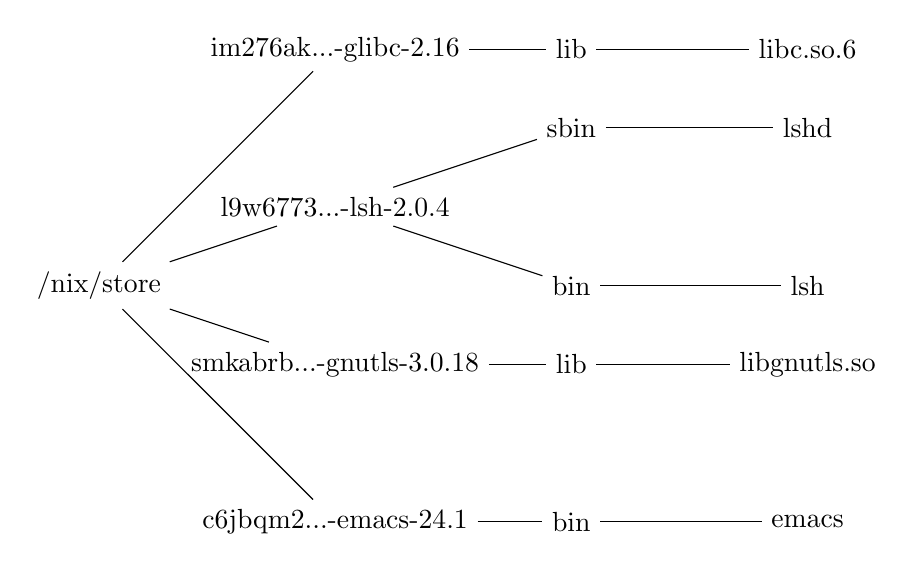
\begin{tikzpicture}
  
    \node {\alert{/nix/store}}
      %[edge from parent fork down, grow=right]
      [grow via three points={%
one child at (3,0) and two children at (3,-1) and (3,1)}]

      child {node {c6jbqm2...-\alert{emacs}-24.1}
        child {node {bin}
          child {node {emacs}}}}
      child {node {smkabrb...-\alert{gnutls}-3.0.18}
        child {node {lib}
          child {node {libgnutls.so}}}}
      child {node {l9w6773...-\alert{lsh}-2.0.4}
        child {node {bin}
          child {node {lsh}}}
        child {node {sbin}
          child {node {lshd}}}}
      child {node {im276ak...-\alert{glibc}-2.16}
        child {node {lib}
          child {node {libc.so.6}}}};

  \end{tikzpicture}
\end{frame}

\begin{frame}
  \frametitle{user environments}

  \begin{overlayarea}{\textwidth}{8cm}
    {
      \small
      \input{nix-user-envs.ltx}
    }

    \only<2-5>{\alert<2>{\code{nix-env --upgrade openssh}}}
    \only<6>{\alert{\code{nix-env --remove-generations old}}}
    \only<7>{\alert{\code{nix-collect-garbage}}}

  \end{overlayarea}

\end{frame}

\begin{frame}[fragile]
  \frametitle{store paths}

  \begin{semiverbatim}
\$ nix-build -A guile
\uncover<2->{/nix/store/\tikz[baseline]{\node[anchor=base](nixhash){\alert<2>{h2g4sc09h4...}};}-guile-2.0.6}

\uncover<3->{\$ \alert<3>{nix-store -q --requisites `which guile`}
/nix/store/4jl83jgzaac...-glibc-2.16
/nix/store/iplay43cg58...-libunistring-0.9.3
/nix/store/47p47v92cj9...-libffi-3.0.9
/nix/store/drkwck2j965...-gmp-5.0.5
...}

\uncover<4->{\$ \alert<4>{nix-copy-closure --to alice@example.com `which guile`}
...}
  \end{semiverbatim}

  \begin{textblock}{7}(5, 10)
    \only<2>{\tikz{\node(labelnixhash){hash of \emph{all} the dependencies};}}
  \end{textblock}

  % Arrows
  \only<2>{
    \begin{tikzpicture}[overlay]
      \path[->](labelnixhash.north) edge (nixhash.south);
    \end{tikzpicture}
  }

\end{frame}

\begin{frame}
  \frametitle{\emph{complete} dependency specification}

  \begin{center}
    \tikz \node(hellobuilddeps){\only<1-2>{\includegraphics[width=1.0\textwidth]{images/hello-buildtime-deps}}\only<3->{\includegraphics[width=0.5\textwidth]{images/hello-runtime-deps}}};
    \\
    \only<2>{\textbf{... down to the compiler's compiler!}}\uncover<3->{\textbf{run-time dependencies \alert{inferred} by conservative scanning}}
  \end{center}

  \begin{textblock}{6}(7, 2)
    \tikz \node(hellobuilddepslabel){\only<1-2>{build}\only<3->{run}-time dependencies of GNU Hello};
  \end{textblock}

  \begin{tikzpicture}[overlay]
    \only<1-2>{\path[->](hellobuilddepslabel.south) edge [bend left] (hellobuilddeps.north);}
  \end{tikzpicture}

\end{frame}

%% \begin{frame}[fragile]
%%   \frametitle{Primitive Build Recipes (a.k.a. ``Nix Expressions'')}

%%   \small{
%%     \begin{semiverbatim}
%% \uncover<2->{\alert{let} dep = }\alert{derivation} \{
%%   name = "foo";
%%   system = "x86\_64-linux";
%%   builder = builtins.toFile "builder.sh"
%%     '' mkdir -p "$out"
%%        echo "Hello, world!" > "$out/some-result"
%%     '';
%% \}\uncover<2->{;}\uncover<3->{ in \alert{derivation} \{
%%   name = "bar";
%%   system = "x86\_64-linux";
%%   builder = builtins.toFile "builder.sh"
%%     '' mkdir -p "$out"
%%        ln -s "\alert{$\{dep\}}/some-result" "\$out/my-result"
%%     '';
%% \} }
%%     \end{semiverbatim}
%%   }

%% \end{frame}


\begin{frame}[fragile]
  \frametitle{packaging using the Nix language}

  \vspace{1cm}
  \small{
    \begin{semiverbatim}
\{ \tikz[baseline]{\node[anchor=base](formalparams){fetchurl, stdenv};}\only<2->{, \alert{gettext}} \}\tikz[baseline]{\node[anchor=base](colon){:};}

\tikz[baseline]{\node[anchor=base](stdenv){\alert<2>{stdenv}};}.\tikz[baseline]{\node[anchor=base](funcall){\alert<1>{mkDerivation}};} \{
  name = "hello-2.3";
  src = fetchurl \{
    url = mirror://gnu/hello/hello-2.3.tar.bz2;
    sha256 = "0c7vijq8y68...";
  \};
 \uncover<2->{\tikz[baseline]{\node[anchor=base](dep){buildInputs = [ \alert{gettext} ];};}}
 \uncover<3->{\tikz[baseline]{\node[anchor=base](bash){preCheck = "echo 'Test suite coming up!'";};}}
  meta = \{
    description = "Produces a friendly greeting";
    homepage = http://www.gnu.org/software/hello/;
    license = "GPLv3+";
  \};
\}
    \end{semiverbatim}
    }

  \begin{textblock}{5}(10, 3)
    \tikz{\node<1>(labelcolon)[fill=white, text=black]{function definition};}
  \end{textblock}

  \begin{textblock}{5}(8, 5)
    \tikz{\node<1>(labelformalparams)[fill=white, text=black]{formal parameters};}
  \end{textblock}

  \begin{textblock}{5}(11, 6)
    \tikz{\node<1>(labelfuncall)[fill=white, text=black]{function call};}
  \end{textblock}

  \begin{textblock}{5}(10, 10)
    \tikz{\node<2>(labeldep)[fill=white, text=black]{dependency};}
  \end{textblock}

  \begin{textblock}{5}(5, 3)
    \tikz{\node<2>(labelstdenv)[fill=white, text=black]{\texttt{gcc}, \texttt{make}, etc.};}
  \end{textblock}

  \begin{textblock}{5}(11, 9)
    \tikz{\node<3>(labelbash)[fill=white, text=black]{Bash snippet};}
  \end{textblock}

  \begin{tikzpicture}[overlay]
    \path[->]<1>(labelcolon) edge (colon);
    \path[->]<1>(labelfuncall) edge (funcall);
    \path[->]<1>(labelformalparams) edge (formalparams);

    \path[->]<2>(labeldep) edge (dep);
    \path[->]<2>(labelstdenv) edge (stdenv);

    \path[->]<3>(labelbash) edge (bash);
  \end{tikzpicture}
\end{frame}

\begin{frame}[fragile]
  \frametitle{package composition with the Nix language}
  \framesubtitle{\texttt{all-packages.nix}}

  \vspace{1cm}
  \begin{semiverbatim}
\alert{gettext} = import ../development/libraries/gettext\tikz{\node(funcall2){};} \{
  inherit \tikz[baseline]{\node[anchor=base](actualparams1){fetchurl stdenv libiconv;};}
\};

\textrm{...}

\alert{hello} = import ../applications/misc/hello\tikz{\node(funcall3){};} \{
  inherit \tikz[baseline]{\node[anchor=base](actualparams2){fetchurl stdenv};};
\};
  \end{semiverbatim}

  \begin{textblock}{5}(5, 9)
    \tikz{\node<1>(labelactualparams)[fill=white, text=black]{actual parameters};}
  \end{textblock}

  \begin{textblock}{5}(13, 9)
    \tikz{\node<1>(labelfuncall2)[fill=white, text=black]{function call};}
  \end{textblock}

  \begin{tikzpicture}[overlay]
    \path[->]<1->(labelactualparams) edge (actualparams1);
    \path[->]<1->(labelactualparams) edge (actualparams2);
    \path[->]<1->(labelfuncall2) edge (funcall2);
    \path[->]<1->(labelfuncall2) edge (funcall3);
  \end{tikzpicture}
\end{frame}

\begin{frame}[fragile]{}

  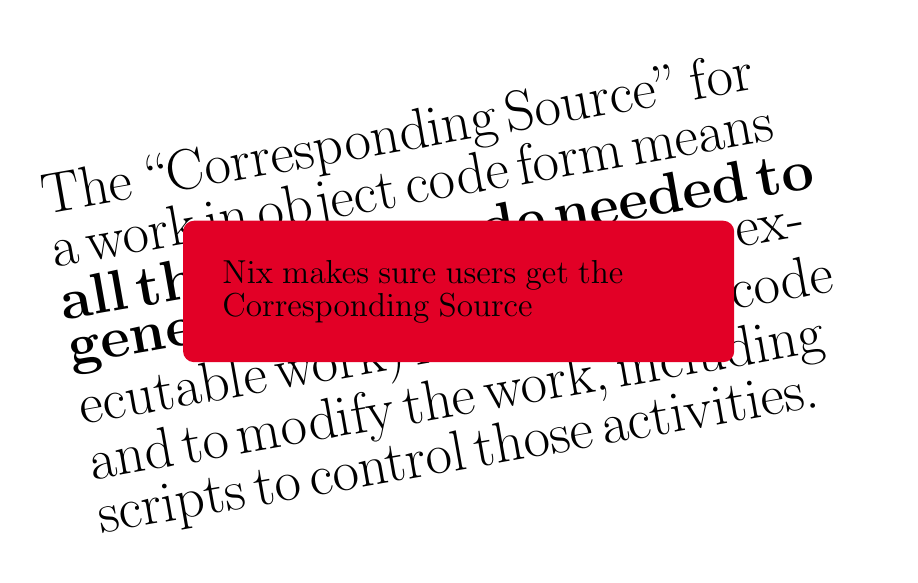
\begin{tikzpicture}
    \node[rotate=10, text width=10cm]{ \huge{\textrm{The
          ``Corresponding Source'' for a work in object code form means
          \alert{\textbf{all the source code needed to generate}},
          install, and (for an executable work) run the object code and
          to modify the work, including scripts to control those
          activities.}}};
    \node<2->[fill=guixred1, inner sep=5mm, text width=6cm,
    rounded corners=4]{\large{Nix makes sure users get the
      Corresponding Source}};
  \end{tikzpicture}
\end{frame}

\subsection{putting it another way}

\begin{frame}
  \vspace{1cm}
  \center{\textbf{Nix implements a \emph{functional} software deployment model.}}

  \vspace{1cm}
  \begin{itemize}
    \item<2-> \alert{\bf immutable} software installations
    \item<3-> builds/installs have \alert{\bf no side effects}
    \item<4-> build \& deployment $\equiv$ calling the build function
    \item<4-> Nix store $\equiv$ \alert{\bf cache} of function call results
    \item<5-> garbage collection...
  \end{itemize}
\end{frame}

%%%%%%%%%%%%%%%%%%%%%%%%%%%%%%%%%%%%%%%%%%%%%%%%%%%%%%%%%%%%%%%%%%%%%%%%%%%%%%%%
\section{from Nix to Guix}

\subsection{rationale}

\begin{frame}{so what's the point of Guix?}
  \huge{keeping Nix's \textbf{build \& deployment model}\\[3.5mm]
    \uncover<2->{using \textbf{Scheme} as the packaging language}\\[3.5mm]
    \uncover<3->{adding \textbf{GNU hackers} to the mix}}
\end{frame}

\begin{frame}{why Guile Scheme instead of the Nix language?}
  \begin{itemize}
  \item<1-> because it rocks!
  \item<2-> because it's GNU!
  \item<3-> it has a compiler, Unicode, gettext, libraries, etc.
  \item<4-> it supports \textbf{embedded DSLs} via macros
  \item<5-> can be used both for composition \emph{and} build scripts
  \end{itemize}
\end{frame}

\subsection{using it}

\begin{frame}[fragile]{Guix's declarative packaging layer}
  \begin{semiverbatim}
    \vspace{-0.5cm}
    \small{
(define-public hello
  (\alert{package}
   (name "hello")
   (version "2.8")
   (source (\alert{origin}
            (method http-fetch)
            (uri (string-append
                  "http://ftp.gnu.org/\textrm{...}/hello-" version
                  ".tar.gz"))
            (sha256 (base32 "0wqd\textrm{...}dz6"))))
   (\alert{build-system} \tikz[baseline]{\node[anchor=base](gbs){gnu-build-system};})
   (arguments '(#:configure-flags '("--disable-silent-rules")))
   \tikz[baseline]{\node[anchor=base](deps){(inputs `(("gawk" ,\tikz[baseline]{\node[anchor=base](gawkvar){\only<1-3,5->{\alert<3>{gawk}}\only<4>{\alert{my-other-awk}}};})))};}
   (description "GNU Hello")
   (long-description "GNUten Tag, Düsseldorf!")
   (home-page "http://www.gnu.org/software/hello/")
   (license "GPLv3+")))
}
  \end{semiverbatim}

  \begin{textblock}{5}(11, 12)
    \tikz{\node<2-3>(labeldeps)[fill=white, text=black]{dependencies};}
  \end{textblock}

  \begin{textblock}{5}(8, 10)
    \tikz{\node<3-4>(labelgawkvar)[fill=white, text=black]{reference to a
        variable};}
  \end{textblock}

  \begin{textblock}{5}(3, 5)
    \tikz{\node<5->(labelgbs)[fill=white, text=black]{\texttt{./configure
        \&\& make install}...};}
  \end{textblock}

  \begin{textblock}{5}(8, 7)
    \tikz{\node<6>(labelgbsdeps)[fill=white, text=black]{depends on
        \texttt{gcc}, \texttt{make}, \texttt{bash}, etc.};}
  \end{textblock}

  \begin{tikzpicture}[overlay]
    \path[->, fill=white, thick]<2-3>(labeldeps) edge (deps);
    \path[->, fill=white, thick]<3-4>(labelgawkvar) edge (gawkvar);
    \path[->, fill=white, thick]<5->(labelgbs) edge (gbs);
    \path[->, fill=white, thick]<6->(labelgbsdeps) edge (gbs);
  \end{tikzpicture}
\end{frame}

\begin{frame}[fragile]{customized package declaration}
  \begin{semiverbatim}
    \vspace{-1.3cm}
    \small{
(define-public gawk
  (\alert{package}
   (name "gawk")
   (version "4.0.0")
   (source (origin (method http-fetch)
                   (uri "http://ftp.gnu.org/...")
                   (sha256 (base32 "0sss..."))))
   (build-system gnu-build-system)
   (\alert{arguments}
     (case-lambda
       ((\tikz[baseline]{\node[anchor=base](sys){system};})                \alert{; native builds}
        (if (string=? system "i686-cygwin")
            '(#:tests? #f)      ; work around test failure
            '(#:parallel-tests? #f))) ; seq. test suite
       ((system cross-system)   \alert{; cross builds}
        (arguments cross-system)))) ; same as above
   (inputs `(("libsigsegv" ,libsigsegv)))
   (home-page "http://www.gnu.org/software/gawk/")
   (description "GNU Awk")))
   }
 \end{semiverbatim}

  \begin{textblock}{5}(8, 7)
    \tikz{\node<2>(labelsys)[fill=white, text=black]{build options
        based on target};}
  \end{textblock}

  \begin{tikzpicture}[overlay]
    \path[->, fill=white, thick]<2>(labelsys) edge (sys);
  \end{tikzpicture}
\end{frame}

\begin{frame}[fragile]{customized package declaration}
  \begin{semiverbatim}
    \vspace{-1.3cm}
    \small{
(define-public guile-1.8
  (\alert{package} \textrm{...}
   (\alert{arguments}
     '(\alert<1>{#:configure-flags} '("--disable-error-on-warning")
       \uncover<2->{\alert<2>{#:patches} (list (assoc-ref %build-inputs "patch/snarf"))}

       \uncover<3->{
       \alert<3-4>{#:phases}
         (\tikz[baseline]{\node[anchor=base](alistcons){alist-cons-before 'configure 'patch-search-path};}
            (lambda* (#:key outputs #:allow-other-keys)
              (\tikz[baseline]{\node[anchor=base](subst){\alert<5>{substitute*}};} "libguile/dynl.c"
                (("lt_dlinit.*\$" match)
                 (format \#f
                   "  ~a~\%  lt\_dladdsearchdir(\\"~a/lib\\");~\%"
                   match (assoc-ref outputs "out")))))
            \tikz[baseline]{\node[anchor=base](phases){\alert<3-4>{\%standard-phases}};})}))
   (inputs `(\uncover<2->{("\alert<2>{patch/snarf}" "distro/guile-1.8.patch")}
             ("gawk" ,gawk)
             ("readline" ,readline)))

   ...
   }
 \end{semiverbatim}

  \begin{textblock}{5}(1, 9)
    \tikz{\node<3-4>[fill=white, text=black](labelphases){configure, build, check, install};}
  \end{textblock}

  \begin{textblock}{5}(8, 5)
    \tikz{\node<4>(labelalistcons)[fill=white, text=black]{add a phase
        before \texttt{configure}};}
  \end{textblock}

  \begin{textblock}{5}(5, 5)
    \tikz{\node<5>(labelsubst)[fill=white, text=black]{patch things up à
        la \texttt{sed}};}
  \end{textblock}

  \begin{tikzpicture}[overlay]
    \path[->, fill=white, thick]<3-4>(labelphases) edge (phases);
    \path[->, fill=white, thick]<4>(labelalistcons) edge (alistcons);
    \path[->, fill=white, thick]<5>(labelsubst) edge (subst);
  \end{tikzpicture}
\end{frame}

\begin{frame}[fragile]{building packages}
  \begin{semiverbatim}
(\alert{use-modules} (guix packages) (guix store)
             (distro base))

(define store
  \tikz[baseline]{\node[anchor=base](conn){(\alert<1>{open-connection})};})

(package? hello)
=> \#t

\uncover<2->{(define drv (\tikz[baseline]{\node[anchor=base](drv){\alert<2>{package-derivation}};} store hello))
\uncover<3->{drv
=> "/nix/store/xyz\textrm{...}-hello-2.8\alert<3>{.drv}"

\uncover<4->{(build-derivations (list drv))
\textsf{\alert{... Nix daemon builds/downloads package on our behalf...}}
\uncover<5->{=> "/nix/store/pqr\textrm{...}-hello-2.8"}}}}
  \end{semiverbatim}

  \begin{textblock}{6}(8, 4)
    \tikz{\node<1>[fill=white, text=black](labelconn){connect to
        the Nix build daemon};}
  \end{textblock}

  \begin{textblock}{6}(9, 6)
    \tikz{\node<2>[fill=white, text=black, text
      width=4.3cm](labeldrv){compute ``derivation''---i.e., build
        promise};}
  \end{textblock}

  \begin{tikzpicture}[overlay]
    \path[->, fill=white, thick]<1>(labelconn) edge (conn);
    \path[->, fill=white, thick]<2>(labeldrv) edge (drv);
  \end{tikzpicture}
\end{frame}

\begin{frame}[fragile]{building packages}
  \begin{semiverbatim}
\$ \alert<1>{guix-build} hello
\uncover<2->{the following derivations will be built:
   /nix/store/4gy79\textrm{...}-gawk-4.0.0.drv
   /nix/store/7m2r9\textrm{...}-hello-2.8.drv
\textrm{...}
\alert{/nix/store/71aj1\textrm{...}-hello-2.8}
}
\end{semiverbatim}
\end{frame}

\begin{frame}[fragile]{under the hood}
  \begin{semiverbatim}
(let* ((store   \tikz[baseline]{\node[anchor=base](conn){(open-connection)};})
       (builder '(\tikz[baseline]{\node[anchor=base](builder){begin};}
                   (mkdir \%output)
                   (call-with-output-file
                       (string-append \%output "/test")
                     (lambda (p)
                       (display '(hello guix) p)))))
       (drv (\tikz[baseline]{\node[anchor=base](drv){\alert{build-expression->derivation}};}
               store "foo" "x86\_64-linux"
               builder
               '(("HOME" . "/nowhere")))))
  (\tikz[baseline]{\node[anchor=base](build){\alert{build-derivations}};} store (list drv)))
  \end{semiverbatim}

  \begin{textblock}{6}(3, 2)
    \tikz{\node<2>[fill=white, text=black](labelconn){connect to
        the build daemon};}
  \end{textblock}

  \begin{textblock}{6}(8, 2)
    \tikz{\node<3>[fill=white, text=black](labelbuilder){build script,
        to be eval'd in chroot};}
  \end{textblock}

  \begin{textblock}{4}(1, 6)
    \tikz{\node<4>[fill=white, text=black, text width=4cm](labeldrv){compute derivation
        for this builder, system, and env.~vars};}
  \end{textblock}

  \begin{textblock}{6}(1, 9)
    \tikz{\node<5>[fill=white, text=black](labelbuild){build it!};}
  \end{textblock}

  \begin{tikzpicture}[overlay]
    \path[->, fill=white, thick]<2>(labelconn) edge (conn);
    \path[->, fill=white, thick]<3>(labelbuilder) edge (builder);
    \path[->, fill=white, thick]<4>(labeldrv) edge (drv);
    \path[->, fill=white, thick]<5>(labelbuild) edge (build);
  \end{tikzpicture}
\end{frame}

\begin{frame}[fragile]{\texttt{derivation} primitive}
  \begin{semiverbatim}
  (let* ((store (open-connection))
         (builder
          (add-text-to-store store "my-builder.sh"
                             "echo hello > \\"\$out\\""
                             '()))
         (drv
          (\alert{derivation} store "foo" "x86\_64-linux"
                      "/bin/sh" `(,builder)
                      '(("HOME" . "/homeless")
                        ("PATH" . "/nothing:/here"))
                      `((,builder)))))
    (build-derivations store (list drv)))
  \end{semiverbatim}
\end{frame}

\begin{frame}{status}
  \begin{itemize}
  \item good API/language support for builds \& composition
  \item expressive enough to build weird packages
  \item<2-> mini Guix-based distro!
  \item<2-> ... bootstrapped with Nixpkgs
  \end{itemize}
\end{frame}

\begin{frame}{tentative road map}
  \begin{itemize}
  \item user environment builders + \texttt{guix-env} command
  \item Guix distro bootstrapped
  \item Guix support in Hydra
  \item distro supports whole-system configuration
  \item<2-> distro has a name
  \item<3-> \bf{you can help!}
  \end{itemize}
\end{frame}

%%%%%%%%%%%%%%%%%%%%%%%%%%%%%%%%%%%%%%%%%%%%%%%%%%%%%%%%%%%%%%%%%%%%%%%%%%%%%%%% 
% \section{Bonuses}

% \begin{frame}[fragile]
%   \frametitle{Cross-Compilation}

%   \begin{enumerate}
%     \item<1-> define the target system
%     \item<3-> build
%     \item<4-> copy to the target store
%     \item<5-> install on the target
%   \end{enumerate}
%   \vspace{4cm}

%   \begin{textblock}{10}(1, 6)
%     \begin{semiverbatim}
%       \only<1>{
% crossSystem = \{          # GNU/Linux on ARM (SheevaPlug)
%   \alert{config} = "armv5tel-unknown-linux-gnueabi";
%   bigEndian = false;
%   arch = "arm";
%   libc = "glibc";
%   float = "soft";
%   withTLS = true;
%   \alert{platform} = pkgs.platforms.sheevaplug;
% \};
%       }
%     \end{semiverbatim}
%   \end{textblock}

%   \begin{textblock}{10}(1, 6)
%     \begin{semiverbatim}
%       \only<2>{
% crossSystem = \{                   # GNU, a.k.a. GNU/Hurd
%   \alert{config} = "i586-pc-gnu";
%   bigEndian = false;
%   arch = "i586";
%   libc = "glibc";
%   float = "hard";
%   withTLS = true;
%   \alert{platform} = pkgs.platforms.pc;
% \};
%       }
%     \end{semiverbatim}
%   \end{textblock}

%   \begin{textblock}{10}(1, 7)
%     \begin{semiverbatim}
%       \only<3>{
% \$ nix-build -A coreutils.\alert{hostDrv}
% \textrm{...}
%       }
%     \end{semiverbatim}
%   \end{textblock}

%   \begin{textblock}{10}(1, 7)
%     \begin{semiverbatim}
%       \only<4>{
% \$ \alert{nix-copy-closure} --to target@foo /nix/store/...
% \textrm{...}
%       }
%     \end{semiverbatim}
%   \end{textblock}

%   \begin{textblock}{10}(1, 7)
%     \begin{semiverbatim}
%       \only<5>{
% target\$ \alert{nix-env --install} /nix/store/...
% \textrm{...}
%       }
%     \end{semiverbatim}
%   \end{textblock}
% \end{frame}

% \begin{frame}[fragile]
%   \frametitle{System-Wide Regression Testing Using VM Networks}

%   \begin{semiverbatim}
% \only<1-2>{\{ pkgs, ... \}:

% \{
%   \alert{nodes} = \{
%     server = 
%       \{ pkgs, config, ... \}:
%       \{ services.openssh.enable = true; \};
      
%     client = 
%       \{ pkgs, config, ... \}:
%       \{ \only<2>{kernelPackages = pkgs.linuxPackages\_2\_6\_25; }\};
%   \};}\only<3>{
%   \alert{testScript} = ''
%     my \$key=`\${pkgs.openssh}/bin/ssh-keygen -t dsa -f key -N ""`;
    
%     \$\alert{server}->mustSucceed("mkdir -m 700 /root/.ssh");
%     \$\alert{server}->copyFileFromHost("key.pub", "/root/.ssh/authorized\_keys");
    
%     \$\alert{client}->mustSucceed("mkdir -m 700 /root/.ssh");
%     \$\alert{client}->copyFileFromHost("key", "/root/.ssh/id\_dsa");
%     \$\alert{client}->mustSucceed("chmod 600 /root/.ssh/id\_dsa");
    
%     \$\alert{client}->mustSucceed("ssh server 'echo Hello RMLL'");
%   '';
% \}}
%   \end{semiverbatim}

% \end{frame}

% \begin{frame}
%   \frametitle{Continuous Integration with Hydra/Nix}

% \only<1>{\center{30+ GNU packages continuously built}}
% \only<1>{\alert{\url{http://hydra.nixos.org/project/gnu/}}}

% %  \vspace{-1cm}
% \only<2>{\center{\includegraphics[width=1.0\textwidth]{images/hydra-gnutls-jobset}}}
% \only<3>{\center{\includegraphics[width=1.0\textwidth]{images/hydra-gnutls-views}}}
% \only<4>{\center{\includegraphics[width=1.0\textwidth]{images/hydra-gnutls-view}}}
% %\only<3>{\center{\includegraphics[width=1.0\textwidth]{images/hydra-gnutls-build}}}

% \end{frame}

\subsection{a GNU distro?}

\begin{frame}[fragile]{why would GNU need a distro?}
  \begin{itemize}
    \item<1->{\textbf{direct connection} between GNU users \& developers
        \begin{itemize}
        \item direct \alert{bug} stream
        \item direct \alert{release} stream
        \end{itemize}
      }
    \item<2->{\textbf{improved integration \& cooperation}
      \begin{itemize}
      \item GNU hackers \alert{know how} to package their software
      \item if GNU foo x.(y + 1) breaks GNU bar, \alert{address that
          directly}
      \end{itemize}}
    \item<3-> following \textbf{free software distro guidelines}
    \item<4-> \textbf{branding!}
  \end{itemize}
\end{frame}

\begin{frame}{why Guix-based?}
  \begin{itemize}
    \item \textbf{technically superior} model \& features
    \item \textbf{traceable} source-to-binary mapping
    \item extensible, i18n'd
    \item<2-> \textbf{Guile} is the official packaging language? :-)
  \end{itemize}
\end{frame}

%%%%%%%%%%%%%%%%%%%%%%%%%%%%%%%%%%%%%%%%%%%%%%%%%%%%%%%%%%%%%%%%%%%%%%%%%%%%%%%%
\begin{frame}
  \frametitle{summary}

  \bf \huge{parentheses + weird paths}
  \uncover<2->{right, but more importantly...}
\end{frame}

\begin{frame}
  \frametitle{summary}

  \begin{itemize}
  \item \textbf{features}
    \begin{itemize}
    \item per-user, unprivileged installation
    \item transactional upgrades; rollback
    \item full power of Guile to build \& compose packages
    \end{itemize}
  \item \textbf{foundations}
    \begin{itemize}
    \item purely functional package management
    \item traceable package source \& dependencies
    \item completely bootstrapped
    \end{itemize}
  \end{itemize}
\end{frame}

\begin{frame}{}

\vfill{
  \vspace{7cm}
  \texttt{ludo@gnu.org} \hfill{\alert{\url{http://gitorious.org/guix/}}}
}

\end{frame}

\begin{frame}{}

  \vfill{
    \tiny{
      Copyright \copyright{} 2010, 2012 Ludovic Courtès \texttt{ludo@gnu.org}.

      Picture of user environments is: \\
      Copyright \copyright{} 2009 Eelco Dolstra \texttt{e.dolstra@tudelft.nl}.

      Copyright of other images included in this document is held by
      their respective owners.
      \\[3.0mm]
      This work is licensed under the \alert{Creative Commons
        Attribution-Share Alike 3.0} License.  To view a copy of this
      license, visit
      \url{http://creativecommons.org/licenses/by-sa/3.0/} or send a
      letter to Creative Commons, 171 Second Street, Suite 300, San
      Francisco, California, 94105, USA.
      \\
      At your option, you may instead copy, distribute and/or modify
      this document under the terms of the \alert{GNU Free Documentation
        License, Version 1.3 or any later version} published by the Free
      Software Foundation; with no Invariant Sections, no Front-Cover
      Texts, and no Back-Cover Texts.  A copy of the license is
      available at \url{http://www.gnu.org/licenses/gfdl.html}.
    }
  }

\end{frame}


\end{document}

% Local Variables:
% coding: utf-8
% comment-start: "%"
% comment-end: ""
% ispell-local-dictionary: "american"
% compile-command: "rubber --pdf guix-ghm-2012.tex"
% End:
